\documentclass{beamer}
\usetheme{Madrid}
\usepackage{amsmath}
\usepackage{pgfplots}
%\pgfplotsset{compat=1.18}
\usepackage{array}


\title{Income Inequality}
\subtitle{Contemporary Economic Issues: ECON 204}
\author{Muhebullah Karimzada}
\date{Winter 2025}
\begin{document}

\begin{frame}
\titlepage
\end{frame}

% Section 1: Introduction
\section{Introduction}

\begin{frame}{What is Income Inequality?}
Income inequality refers to the unequal distribution of income among individuals or households within a country. In Canada, income inequality has been a growing concern, with disparities between the rich and the poor widening over time.
\end{frame}

% Section 2: Key Definitions
\section{Key Definitions}

\begin{frame}{Key Definitions}
\begin{itemize}
    \item \textbf{Income Inequality}: The gap between the rich and the poor in terms of income distribution.
    \item \textbf{Gini Coefficient}: A measure of income inequality ranging from 0 (perfect equality) to 1 (perfect inequality).
    \item \textbf{Lorenz Curve}: A graphical representation of income distribution.
    \item \textbf{Quintiles}: Dividing the population into five equal groups based on income.
    \item \textbf{Disposable Income}: Income after taxes and transfers.
\end{itemize}
\end{frame}

% Section 3: Income Inequality in Canada
\section{Income Inequality in Canada}

\begin{frame}{Income Inequality in Canada: An Overview}
\begin{itemize}
    \item \textbf{Trends}: Income inequality in Canada has increased since the 1980s.
    \item \textbf{Key Statistics}:
        \begin{itemize}
            \item Top 10\% of earners hold about \textbf{25\%} of total income.
            \item Bottom 50\% of earners hold about \textbf{20\%} of total income.
        \end{itemize}
    \item \textbf{Regional Disparities}: Higher inequality in Ontario and Alberta compared to Atlantic Canada.
\end{itemize}
\end{frame}

% Section 4: Measuring Income Inequality
\section{Measuring Income Inequality}

\begin{frame}{Gini Coefficient}
The Gini coefficient is a numerical measure of income inequality. It is calculated using the Lorenz curve.

\[
\text{Gini Coefficient} = \frac{\text{Area between Lorenz curve and equality line}}{\text{Area under equality line}}
\]
\end{frame}



% Table 3: Income Distribution for Example 2
\begin{frame}{Income Distribution Table: Example }
Consider another income distribution for a hypothetical country:
\begin{table}[h]
\centering
\begin{tabular}{|c|c|}
\hline
\textbf{Income Group} & \textbf{Income Share (\%)} \\
\hline
Bottom 20\% & 10 \\
Next 20\% & 15 \\
Middle 20\% & 20 \\
Next 20\% & 25 \\
Top 20\% & 30 \\
\hline
\end{tabular}
\end{table}

This table shows a more equal distribution of income compared to the previous example.
\end{frame}

% Table 4: Quintiles and Cumulative Shares for Example 2
\begin{frame}{Quintiles and Cumulative Shares: Example }
Using the income distribution table, we calculate the cumulative income shares for each quintile:
\begin{table}[h]
\centering
\begin{tabular}{|c|c|c|}
\hline
\textbf{Quintile} & \textbf{Income Share (\%)} & \textbf{Cumulative Income Share (\%)} \\
\hline
Bottom 20\% & 10 & 10 \\
Next 20\% & 15 & 25 \\
Middle 20\% & 20 & 45 \\
Next 20\% & 25 & 70 \\
Top 20\% & 30 & 100 \\
\hline
\end{tabular}
\end{table}

The cumulative income share is calculated by adding the income share of each quintile to the previous total.
\end{frame}

% Lorenz Curve Plot for Example 2
\begin{frame}{Lorenz Curve: Example }
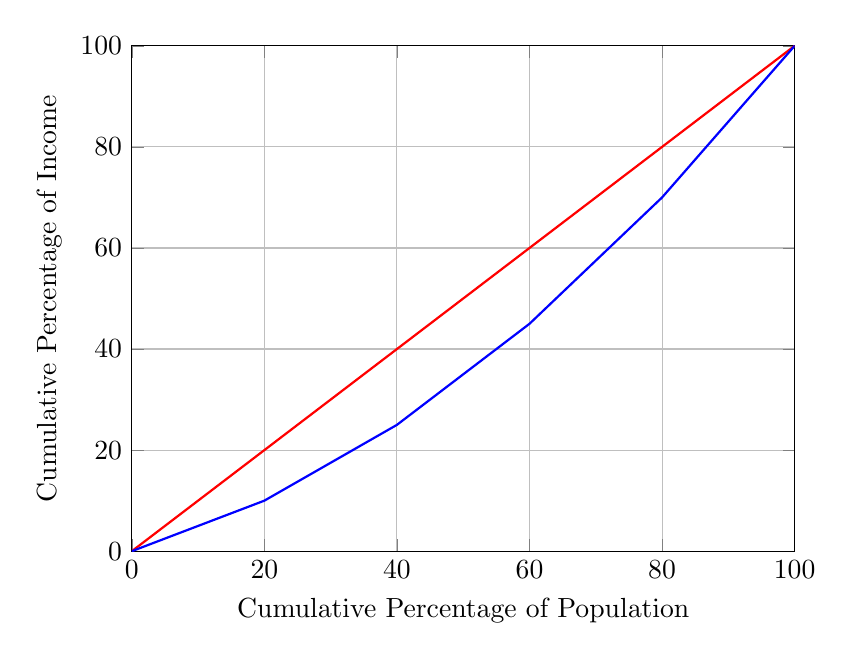
\begin{tikzpicture}
\begin{axis}[
    xlabel={Cumulative Percentage of Population},
    ylabel={Cumulative Percentage of Income},
    xmin=0, xmax=100,
    ymin=0, ymax=100,
    xtick={0,20,40,60,80,100},
    ytick={0,20,40,60,80,100},
    grid=both,
    width=10cm,
    height=8cm,
]
% Line of Equality
\addplot[domain=0:100, red, thick] {x};
% Lorenz Curve
\addplot[blue, thick] coordinates {
    (0, 0)
    (20, 10)
    (40, 25)
    (60, 45)
    (80, 70)
    (100, 100)
};
\end{axis}
\end{tikzpicture}


\end{frame}

% Explanation of the Trapezoidal Rule
\begin{frame}{Trapezoidal Rule}
The trapezoidal rule is a method for approximating the area under a curve by dividing it into trapezoids. For the Lorenz curve, we use the trapezoidal rule to calculate the area under the curve.

\[
\text{Area of a trapezoid} = \frac{1}{2} \times (\text{Base}_1 + \text{Base}_2) \times \text{Height}
\]

In the context of the Lorenz curve:
- \(\text{Base}_1\) and \(\text{Base}_2\) are the cumulative income shares at two consecutive points.
- \(\text{Height}\) is the width of the interval (20\% in this case).
\end{frame}

% Area Calculation: Step 1
\begin{frame}{Area Calculation: Step 1}
1. The area under the line of equality (perfect equality) is:
\[
\text{Area}_{\text{equality}} = \frac{1}{2} \times 100 \times 100 = 5000
\]
This represents the total area under the 45-degree line.
\end{frame}

% Area Calculation: Step 2
\begin{frame}{Area Calculation: Step 2}
2. The area under the Lorenz curve is calculated using the trapezoidal rule:
\begin{scriptsize}

\[
\text{Area}_{\text{Lorenz}} = \frac{1}{2} \times (10 + 25) \times 20 + \frac{1}{2} \times (25 + 45) \times 20 + \frac{1}{2} \times (45 + 70) \times 20 + \frac{1}{2} \times (70 + 100) \times 20 = 3900
\]

\end{scriptsize}
\[
\text{Area}_{\text{Lorenz}} = 350 + 700 + 1150 + 1700 = 3900
\]
\end{frame}

% Area Calculation: Step 3
\begin{frame}{Area Calculation: Step 3}
3. The area between the Lorenz curve and the line of equality is:
\[
\text{Area}_{\text{between}} = \text{Area}_{\text{equality}} - \text{Area}_{\text{Lorenz}} = 5000 - 3900 = 1100
\]
This area represents the degree of income inequality.
\end{frame}

% Area Calculation: Step 4
\begin{frame}{Area Calculation: Step 4}
4. The Gini coefficient is:
\[
\text{Gini Coefficient} = \frac{\text{Area}_{\text{between}}}{\text{Area}_{\text{equality}}} = \frac{1100}{5000} = 0.22
\]
A Gini coefficient of 0.22 indicates low income inequality.
\end{frame}


% Lorenz Curve Plot for Example 2
\begin{frame}{Lorenz Curve: Example }


\begin{small}
\begin{footnotesize}
\textbf{Area Calculation}:
1. The area under the line of equality (perfect equality) is:
\[
\text{Area}_{\text{equality}} = \frac{1}{2} \times 100 \times 100 = 5000
\]
2. The area under the Lorenz curve is calculated using the trapezoidal rule:
\begin{scriptsize}

\[
\text{Area}_{\text{Lorenz}} = \frac{1}{2} \times (10 + 25) \times 20 + \frac{1}{2} \times (25 + 45) \times 20 + \frac{1}{2} \times (45 + 70) \times 20 + \frac{1}{2} \times (70 + 100) \times 20 = 3900
\]

\end{scriptsize}
3. The area between the Lorenz curve and the line of equality is:
\[
\text{Area}_{\text{between}} = \text{Area}_{\text{equality}} - \text{Area}_{\text{Lorenz}} = 5000 - 3900 = 1500
\]
4. The Gini coefficient is:
\[
\text{Gini Coefficient} = \frac{\text{Area}_{\text{between}}}{\text{Area}_{\text{equality}}} = \frac{1100}{5000} = 0.22
\]
\end{footnotesize}
\end{small}
\end{frame}









% Section 5: Causes of Income Inequality
\section{Causes of Income Inequality}

\begin{frame}{Causes of Income Inequality in Canada}
\begin{itemize}
    \item \textbf{Globalization}: Outsourcing of manufacturing jobs.
    \item \textbf{Technological Change}: Automation and AI replacing low-skilled jobs.
    \item \textbf{Education Gap}: Unequal access to quality education.
    \item \textbf{Tax Policies}: Reduction in progressive taxation.
    \item \textbf{Wealth Accumulation}: The rich benefit more from capital gains.
\end{itemize}
\end{frame}

% Section 6: Consequences of Income Inequality
\section{Consequences of Income Inequality}

\begin{frame}{Consequences of Income Inequality in Canada}
\begin{itemize}
    \item \textbf{Economic}: Reduced economic growth due to lower consumption.
    \item \textbf{Social}: Increased crime rates and social unrest.
    \item \textbf{Health}: Poorer health outcomes for low-income groups.
    \item \textbf{Political}: Concentration of political power among the wealthy.
\end{itemize}
\end{frame}

% Section 7: Policy Responses
\section{Policy Responses}

\begin{frame}{Policy Responses to Income Inequality in Canada}
\begin{itemize}
    \item \textbf{Progressive Taxation}: Higher tax rates for higher income brackets.
    \item \textbf{Minimum Wage Laws}: Ensuring a living wage for low-income workers.
    \item \textbf{Education Reform}: Improving access to quality education.
    \item \textbf{Social Safety Nets}: Expanding unemployment benefits and healthcare.
    \item \textbf{Wealth Taxes}: Taxing inherited wealth and capital gains.
\end{itemize}
\end{frame}

% Section 8: Case Study
\section{Case Study}

\begin{frame}{Case Study: Income Inequality in Ontario}
\begin{itemize}
    \item \textbf{Key Facts}:
        \begin{itemize}
            \item Ontario has the highest income inequality among Canadian provinces.
            \item Top 1\% of earners hold about \textbf{12\%} of total income.
        \end{itemize}
    \item \textbf{Causes}:
        \begin{itemize}
            \item Decline in manufacturing jobs.
            \item High cost of living in cities like Toronto.
        \end{itemize}
    \item \textbf{Policy Responses}:
        \begin{itemize}
            \item Higher minimum wage.
            \item Expansion of childcare subsidies.
        \end{itemize}
\end{itemize}
\end{frame}

% Section 9: Future Trends
\section{Future Trends}

\begin{frame}{Future Trends}
\begin{itemize}
    \item \textbf{Automation}: Widening the gap between high-skilled and low-skilled workers.
    \item \textbf{Universal Basic Income (UBI)}: A potential solution to job displacement.
    \item \textbf{Climate Change}: Disproportionately affecting low-income populations.
\end{itemize}
\end{frame}

% Section 10: Conclusion
\section{Conclusion}

\begin{frame}{Conclusion}
Income inequality in Canada is a multifaceted issue with significant economic, social, and political implications. Addressing it requires a combination of progressive taxation, social safety nets, and investments in education and training.
\end{frame}

\end{document}